\documentclass[xetex,mathserif,serif]{beamer}
\usepackage{polyglossia}
\setdefaultlanguage[babelshorthands=true]{russian}
\usepackage{minted}
\usepackage{tabu}

\useoutertheme{infolines}

\usepackage{fontspec}
\setmainfont{FreeSans}
\newfontfamily{\russianfonttt}{FreeSans}

\definecolor{links}{HTML}{2A1B81}
\hypersetup{colorlinks,linkcolor=,urlcolor=links}

\tabulinesep=0.7mm

\newcommand{\attribution}[1] {
    \vspace{-5mm}\begin{flushright}\begin{scriptsize}\textcolor{gray}{\textcopyright\, #1}\end{scriptsize}\end{flushright}
}

\title{Практика 5: моделирование поведения}
\author[Юрий Литвинов]{Юрий Литвинов \newline \textcolor{gray}{\small\texttt{yurii.litvinov@gmail.com}}}

\date{14.02.2022}

\begin{document}

    \frame{\titlepage}

    \section{Диаграммы последовательностей}

    \begin{frame}
        \frametitle{Диаграммы последовательностей}
        \framesubtitle{Sequence diagrams}
        \begin{center}
            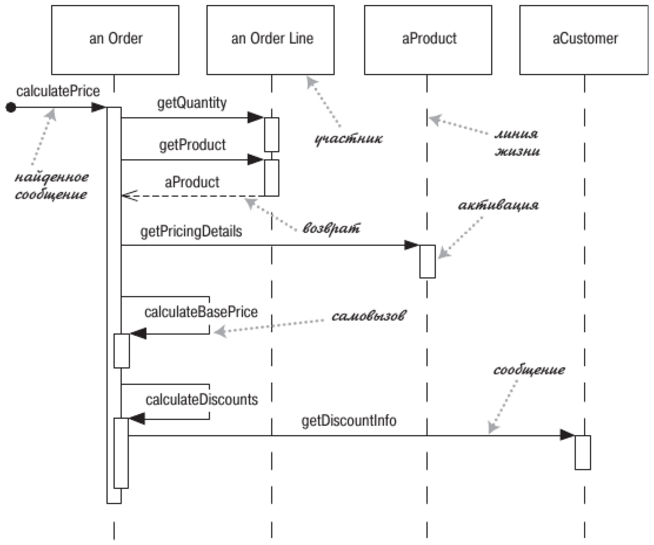
\includegraphics[width=0.6\textwidth]{sequenceDiagram.png}
        \end{center}
    \end{frame}

    \begin{frame}
        \frametitle{Диаграммы последовательностей, создание и удаление объектов}
        \begin{center}
            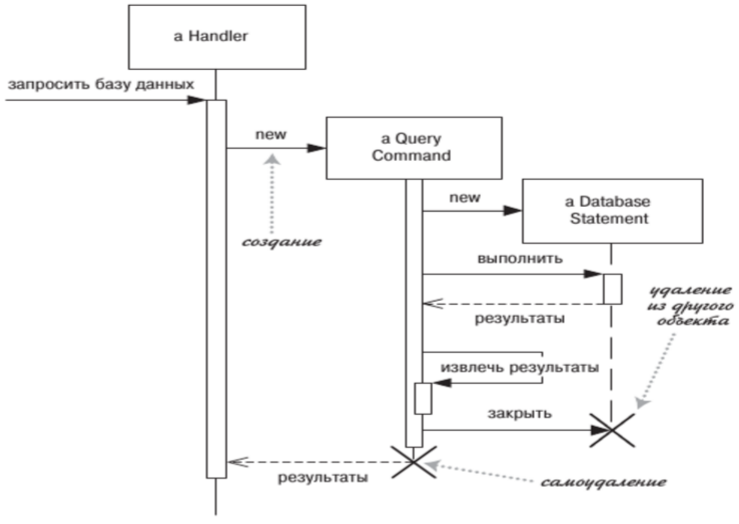
\includegraphics[width=0.65\textwidth]{sequenceLifeCycle.png}
        \end{center}
    \end{frame}

    \begin{frame}
        \frametitle{Диаграммы последовательностей, фреймы}
        \begin{center}
            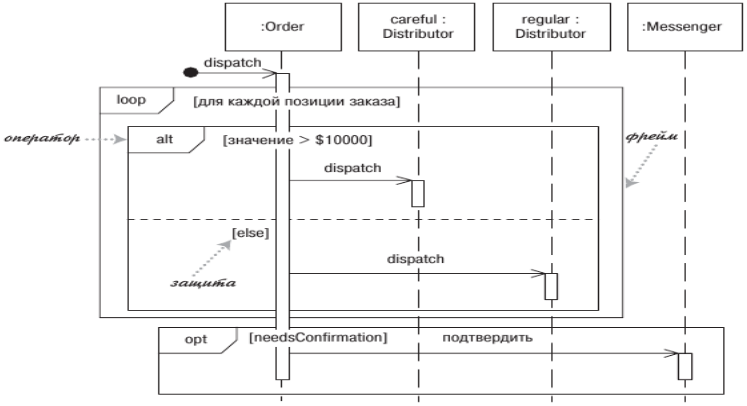
\includegraphics[width=0.8\textwidth]{sequenceFrames.png}
        \end{center}
    \end{frame}

    \section{Диаграммы конечных автоматов}

    \begin{frame}
        \frametitle{Диаграммы конечных автоматов}
        \framesubtitle{Диаграммы состояний}
        \begin{columns}
            \begin{column}{0.4\textwidth}
                \begin{itemize}
                    \item Состояния объекта как часть жизненного цикла
                    \item Моделирование реактивных объектов
                    \begin{itemize}
                        \item Например, сетевое соединение
                    \end{itemize}
                \end{itemize}
            \end{column}
            \begin{column}{0.6\textwidth}
                \begin{center}
                    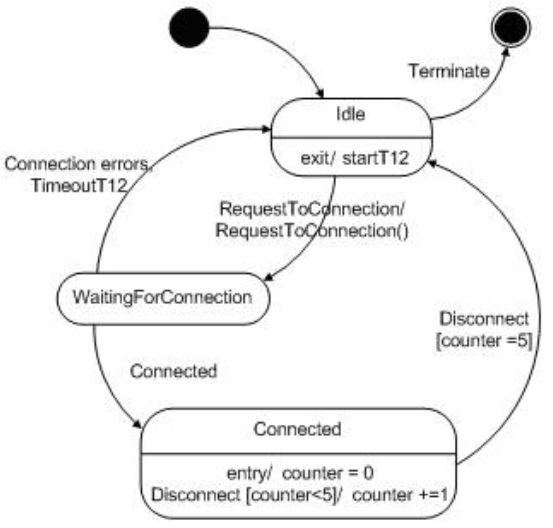
\includegraphics[width=0.7\textwidth]{stateTransitionExample.png}
                \end{center}
            \end{column}
        \end{columns}
    \end{frame}

    \begin{frame}
        \frametitle{Диаграммы конечных автоматов, синтаксис}
        \begin{columns}
            \begin{column}{0.5\textwidth}
                \begin{itemize}
                    \item Состояние
                    \begin{itemize}
                        \item entry activity
                        \item exit activity
                        \item do activity
                        \item внутренний переход
                    \end{itemize}
                    \item Событие
                    \item Переход
                    \begin{itemize}
                        \item имя события (список параметров) [сторожевое условие] выражение действия
                    \end{itemize}
                \end{itemize}
            \end{column}
            \begin{column}{0.5\textwidth}
                \begin{center}
                    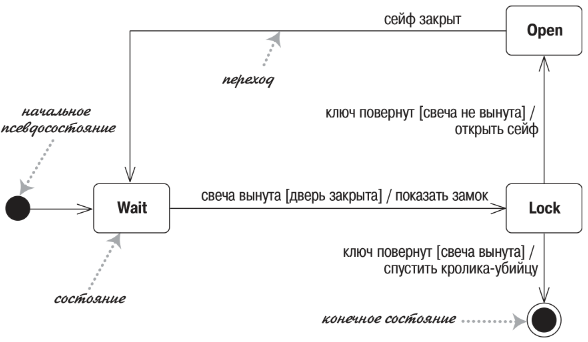
\includegraphics[width=\textwidth]{stateTransitionSyntax.png}
                    \attribution{М. Фаулер, UML. Основы}
                \end{center}
            \end{column}
        \end{columns}
    \end{frame}

    \section{Временные диаграммы}

    \begin{frame}
        \frametitle{Временные диаграммы}
        \begin{columns}
            \begin{column}{0.5\textwidth}
                \begin{center}
                    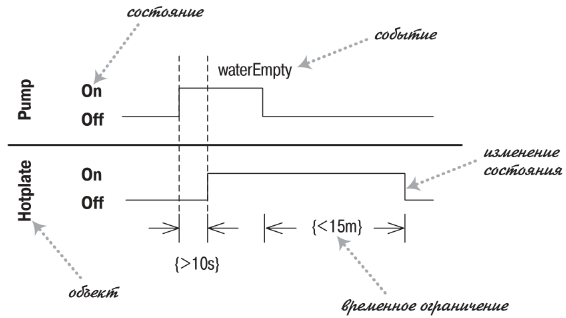
\includegraphics[width=0.9\textwidth]{timingDiagrams.png}
                \end{center}
            \end{column}
            \begin{column}{0.5\textwidth}
                \begin{center}
                    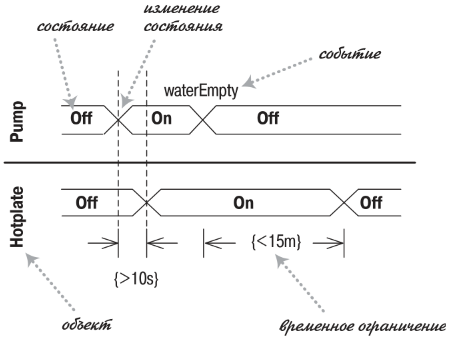
\includegraphics[width=0.8\textwidth]{timingDiagramsAlternate.png}
                    \attribution{М. Фаулер, UML. Основы}
                \end{center}
            \end{column}
        \end{columns}
    \end{frame}

    \section{Задачи на остаток пары}

    \begin{frame}
        \frametitle{Задание на остаток пары}
        Нарисовать следующие диаграммы:
        \begin{enumerate}
            \item диаграмму последовательностей регистрации и ремонта дефекта из уже знакомого вам запроса \url{https://bit.ly/defects-rfp};
            \item диаграмму конечных автоматов, описывающую поведение микроволновки;
            \item временную диаграмму любого сценария работы микроволновки;
            \begin{itemize}
                \item в VP это может быть не совсем тривиально: \url{https://www.visual-paradigm.com/support/documents/vpuserguide/94/2586/6715_drawingtimin.html}
                \item в diagrams.net не факт, что вообще возможно, из браузерных решений, наверное \url{https://creately.com/lp/timing-diagram-software/}
            \end{itemize}
        \end{enumerate}
    \end{frame}

\end{document}
